
\subsection*{2.6 Quadratic Equations and Inequalities}
Quadratic equations and inequalities involve a variable raised to the second power. They are fundamental in algebra and appear in various real-world applications.

\textbf{Key Concepts:}
\begin{itemize}
    \item \textbf{General Form of a Quadratic Equation:}
    \[
    ax^2 + bx + c = 0, \quad a \neq 0
    \]
    where $a$, $b$, and $c$ are constants.
    \item \textbf{Quadratic Formula:} Used to solve quadratic equations:
    \[
    x = \frac{-b \pm \sqrt{b^2 - 4ac}}{2a}.
    \]
    \item \textbf{Ways to Solve Quadratic Equations:}
    \begin{itemize}
        \item By factorization.
        \item By completing the square.
        \item By using the quadratic formula.
    \end{itemize}
    \item \textbf{Discriminant:} The discriminant $\Delta = b^2 - 4ac$ determines the nature of the roots:
    \begin{itemize}
        \item If $\Delta > 0$, there are two distinct real roots.
        \item If $\Delta = 0$, there is one real root (a repeated root).
        \item If $\Delta < 0$, there are no real roots (two complex roots).
    \end{itemize}
    \item \textbf{Graph of a Quadratic Function:} The graph of $y = ax^2 + bx + c$ is a parabola:
    \begin{itemize}
        \item If $a > 0$, the parabola opens upwards.
        \item If $a < 0$, the parabola opens downwards.
        
        \begin{figure}[h!]
     \centering
    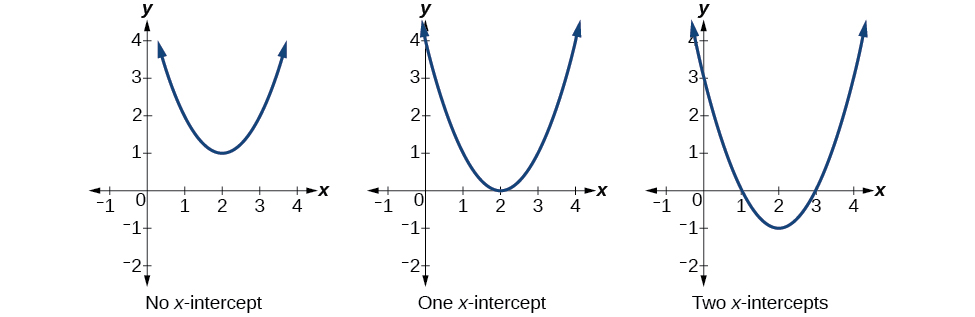
\includegraphics[width=0.8\textwidth]{2.1.png}
    \caption{Three cases for quadratic graph, depending on discriminant.}
    \label{fig:your-label}
\end{figure}
    \end{itemize}
    The vertex is given by:
    \[
    x = -\frac{b}{2a}.
    \]
    \item \textbf{Vieta's Formulas for Roots:}
    \begin{itemize}
        \item Sum of roots: $r_1 + r_2 = -\frac{b}{a}$.
        \item Product of roots: $r_1 \cdot r_2 = \frac{c}{a}$.
    \end{itemize}
    \item \textbf{Constructing a Quadratic Equation from Given Roots:}  
If the roots of a quadratic equation are \( \alpha \) and \( \beta \), then the equation can be formed using Vieta's formula:
\[
x^2 - (\alpha + \beta)x + \alpha\beta = 0
\]
This formula uses the sum and product of the roots to construct the quadratic equation. See Example 5.

\end{itemize}

\begin{flushleft}
\textbf{Example 1: Solve $x^2 - 5x + 6 = 0$ by factorization.}

\vspace{0.5cm}
\textbf{Solution:}
\vspace{0.5cm}

Step 1: Factorize the quadratic equation:
\[
x^2 - 5x + 6 = (x - 2)(x - 3).
\]

Step 2: Solve for $x$:
\[
x - 2 = 0 \implies x = 2, \quad x - 3 = 0 \implies x = 3.
\]

Therefore, the solutions are $x = 2$ and $x = 3$.
\end{flushleft}

\begin{flushleft}
\textbf{Example 2: Solve $x^2 + 6x + 5 = 0$ by completing the square.}

\vspace{0.5cm}
\textbf{Solution:}
\vspace{0.5cm}

Step 1: Rewrite the equation:
\[
x^2 + 6x = -5.
\]

Step 2: Complete the square:
\[
x^2 + 6x + 9 = -5 + 9 \implies (x + 3)^2 = 4.
\]

Step 3: Solve for $x$:
\[
x + 3 = \pm \sqrt{4} \implies x + 3 = 2 \quad \text{or} \quad x + 3 = -2.
\]

Step 4: Simplify:
\[
x = -1 \quad \text{or} \quad x = -5.
\]

Therefore, the solutions are $x = -1$ and $x = -5$.
\end{flushleft}

\begin{flushleft}
\textbf{Example 3: Solve $2x^2 - 3x + 1 = 0$ using the quadratic formula.}

\vspace{0.5cm}
\textbf{Solution:}
\vspace{0.5cm}

Identify the coefficients:
\[
a = 2, \quad b = -3, \quad c = 1.
\]

Use the quadratic formula:
\[
x = \frac{-(-3) \pm \sqrt{(-3)^2 - 4(2)(1)}}{2(2)}.
\]

Simplify:
\[
x = \frac{3 \pm \sqrt{9 - 8}}{4} = \frac{3 \pm 1}{4}.
\]

Solve for $x$:
\[
x = \frac{3 + 1}{4} = 1 \quad \text{or} \quad x = \frac{3 - 1}{4} = \frac{1}{2}.
\]

Therefore, the solutions are $x = 1$ and $x = \frac{1}{2}$.
\end{flushleft}

\begin{flushleft}
\textbf{Example 4: Find the nature of the roots for $x^2 + 4x + 5 = 0$.}

\vspace{0.5cm}
\textbf{Solution:}
\vspace{0.5cm}

Step 1: Calculate the discriminant:
\[
\Delta = b^2 - 4ac = 4^2 - 4(1)(5) = 16 - 20 = -4.
\]

Step 2: Interpret the result:
\[
\Delta < 0 \implies \text{the equation has two complex roots.}
\]

Therefore, the roots are complex.
\end{flushleft}

\begin{flushleft}
\textbf{Example 5: Write a quadratic equation whose roots are $-\frac{1}{2}$ and $3$.}

\vspace{0.5cm}
\textbf{Solution:}
\vspace{0.5cm}

Step 1: Use Vieta's formulas for roots:
\[
\text{Sum of roots: } r_1 + r_2 = -\frac{b}{a}.
\]
\[
\text{Product of roots: } r_1 \cdot r_2 = \frac{c}{a}.
\]

Step 2: Substitute the given roots $r_1 = -\frac{1}{2}$ and $r_2 = 3$:
\[
\text{Sum of roots: } -\frac{1}{2} + 3 = \frac{5}{2}.
\]
\[
\text{Product of roots: } \left(-\frac{1}{2}\right)(3) = -\frac{3}{2}.
\]

Step 3: Write the quadratic equation using the general form:
\[
a \cdot x^2 - (\text{sum of roots}) \cdot x + (\text{product of roots}) = 0.
\]

Substitute the values and assuming a=1 for the simplest case:
\[
x^2 - \frac{5}{2}x - \frac{3}{2} = 0.
\]

Step 4: Eliminate fractions by multiplying through by 2:
\[
2x^2 - 5x - 3 = 0.
\]

Therefore, the quadratic equation is $2x^2 - 5x - 3 = 0$.
\end{flushleft}

